% !TeX root=main.tex

\pagenumbering{arabic}

\chapter{مقدمه}
%\thispagestyle{empty}
\section{شرح مسئله}
{
در سال‌های اخیر پیشرفت‌های زیادی در مسائل هوش مصنوعی و یادگیری عمیق که در تقاطع دو حوزه پردازش زبان طبیعی  و بینایی ماشین  قرار می‌گیرند؛ رخ داده است. یکی از مسائلی که اخیراً مورد توجه قرارگرفته است؛ پرسش و پاسخ تصویری  است. با توجه به یک تصویر و یک سؤال به زبان طبیعی، سیستم سعی می‌کند با استفاده از عناصر بصری تصویر و استنتاج جمع آوری شده از سوال متنی، پاسخ صحیح را پیدا کند. پرسش و پاسخ تصویری نسخه گسترش یافته مسئله پرسش و پاسخ متنی  است است که اطلاعات بصری به مسئله اضافه شده است. شکل \ref{fig:VQAExample}  گویای تفاوت این دو مسئله است.
	\begin{figure}
		\centerline{
			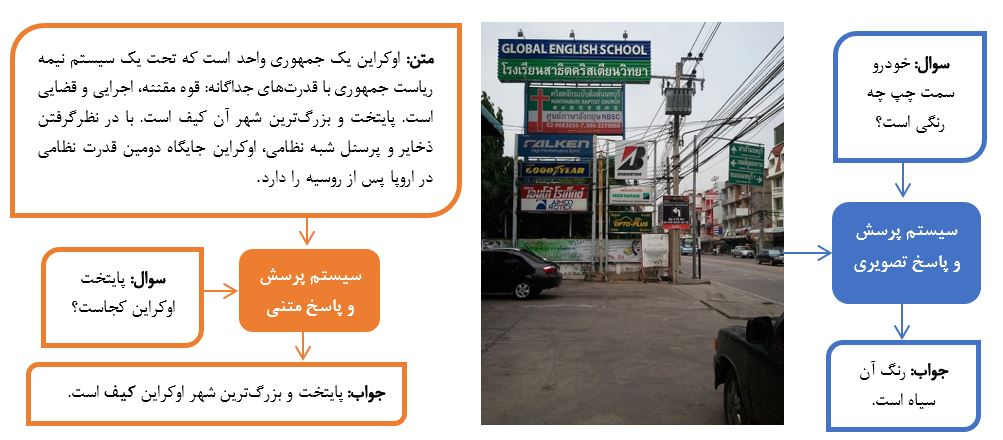
\includegraphics[scale=0.7]{images/1.JPG}}
		\caption{مثالی از سیستم پرسش و پاسخ متنی و تصویری}
		\label{fig:VQAExample}
	\end{figure}
	
	در سیستم پرسش و پاسخ متنی، یک متن و یک سوال متنی به عنوان ورودی به سیستم داده می‌شود و انتظار می‌رود که سیستم با توجه به درک و تفسیری که از متن و سوال بدست می‌آورد؛ یک جواب متنی را خروجی دهد. اما در سیستم پرسش و پاسخ تصویری، یک تصویر و یک سوال متنی به ورودی سیستم داده می‌شود و انتظار می‌رود که سیستم بتواند با استفاده از عناصر بصری تصویر و تفسیری که از سوال بدست می‌آورد؛ یک پاسخ متنی را در خروجی نشان دهد.
	
	مسئله پرسش و پاسخ تصویری پیچیدگی بیشتری نسبت به مسئله پرسش و پاسخ متنی دارد زیرا تصاویر بعد بالاتر و نویز بیشتری نسبت به متن دارند. علاوه بر این، تصاویر فاقد ساختار و قواعد دستوری زبان هستند. در نهایت هم، تصاویر غنای بیشتری از دنیای واقعی را ضبط می‌کنند، در حالی که زبان طبیعی در حال حاضر نشانگر سطح بالاتری از انتزاع دنیای واقعی است. 
	
}
\section{کاربرد و اهمیت مسئله}
{
در طی سال‌های متمادی، محققان به دنبال ساخت ماشین‌هایی بودند که به اندازه‌ی کافی باهوش باشند که از آن به طور موثر همانند انسان‌ها برای تعامل استفاده کنند. مسئله‌ی پرسش و پاسخ تصویری یکی از پله‌های رسیدن به این رویای هوش مصنوعی است و از این جهت حائز اهمیت است.

کاربردهای بسیاری برای پرسش و پاسخ تصویری وجود دارد. یکی از مهم‌ترین موارد دستیار هوشمند برای افراد کم‌بینا و نابینا  است. علاوه بر این، در سال های اخیر دستیاران صوتی  و عامل‌های گفتگو  مانند  
\lr{Cortana}
،
\lr{Siri}
و
\lr{Alexa}
  در بازار عرضه شدند که می‌توانند با انسان‌ها با استفاده از زبان طبیعی ارتباط برقرار کنند. در حال حاضر این دستیاران با استفاده از صوت و متن این ارتباط را برقرار می‌کنند در نتیجه گفتگوی بین این دستیاران با انسان‌ها مشابه دنیای واقعی نمی‌باشد. این ارتباط را می‌توان با استفاده از داده‌های تصویری و ویدئویی به واقعیت نزدیک‌تر کرد. اینجاست که مسئله‌ی پرسش و پاسخ تصویری برای نزدیک کردن تعامل بین انسان و عامل‌های گفتگو به دنیای واقعی می‌تواند موثر باشد.  همین موضوع را می‌توانیم به صورت گسترده‌تری در ربات‌ها مشاهده کنیم. برای این‌که ربات بتواند بهتر با انسان‌ها ارتباط برقرار کند و به سوالات و درخواست‌ها پاسخ دهد؛ نیاز دارد که درک و فهم درستی از اطراف داشته باشد که این مستلزم داشتن تصویری دقیق از پیرامون است. بنابراین این ربات می‌تواند برای پاسخ به پرسش‌ها از دانشی که از طریق تصویر پیرامون خود بدست می‌آورد، جواب درستی را بدهد.
  
  کاربرد دیگر این مسئله در پزشکی است. در بسیاری از موارد تحلیل تصاویر پزشکی مانند تصاویر CT‌ اسکن و x-ray برای یک پزشک متخصص هم دشوار است. اما یک سیستم پرسش و پاسخ تصویری می‌تواند با تحلیل و تشخیص موارد غیرطبیعی موجود در تصویر، به عنوان نظر دوم به پزشک متخصص کمک کند. از طرفی ممکن است در بعضی اوقات بیمار دسترسی به پزشک را نداشته باشد تا شرح تصاویر را متوجه شود. وجود سیستم پرسش و پاسخ تصویری می‌تواند آگاهی بیمار را نسبت به بیماری افزایش دهد و از نگرانی او بکاهد.
}
\section{بررسی چالشهای موجود در این مسئله}
باید تکمیل شود.
\section{بررسی مجموعه دادگان مطرح و مسابقات مطرح این حوزه}
در این بخش به معرفی مجموعه‌داده‌های مشهور در حوزه‌ی پرسش و پاسخ تصویری می‌پردازیم و ویژگی‌های هر کدام را بررسی خواهیم کرد. 
\begin{table}
	\begin{center}
		\begin{tabular}{ |c|c|c|c| } 
			\hline
			\textbf{مجموعه‌داده} & \textbf{تعداد تصاویر} & \textbf{تعدادسوالات} & \textbf{سال انتشار} \\
			\hline \hline
			\textbf{\lr{DAQUAR}} & 1449 & 12468 & 2014 \\
			\hline
			\textbf{\lr{VQA v1}} & 204721 & 614163 & 2015 \\
			\hline
			\textbf{\lr{VQA v2}} & 0 & 0 & 0 \\
			\hline
			\textbf{\lr{Visual Madlibs}} & 10738 & 360001 & 2015 \\
			\hline
			\textbf{\lr{Visual7w}} & 47300 & 2201154 & 2016 \\
			\hline
			\textbf{\lr{CLEVR}} & 100000 & 853554 & 2017 \\
			\hline
			\textbf{\lr{Tally-QA}} & 165000 & 306907 & 2019 \\
			\hline
			\textbf{\lr{KVQA}} & 24602 & 183007 & 2019 \\
			\hline
		\end{tabular}
	\end{center}
	\caption{بررسی اجمالی مجموعه‌داده‌های معروف در حوزه پرسش و پاسخ تصویری.}
	\label{tabel:1}
\end{table}
در جدول 
\ref{tabel:1}
اطلاعات آماری این مجموعه‌داده‌ها به صورت خلاصه آمده‌است.
\subsection{مجموعه داده \lr{DAQUAR}}
{
	\textbf{DAQUAR}
	 مخفف
	\lr{Dataset for Question Answering on Real World Images}
است که توسط مالینوفسکی منتشر‌شده‌است. این اولین مجموعه‌داده‌ای است که برای مسئله 
	\lr{VQA}
 منتشر‌شده‌است. تصاویر از مجموعه‌داده
  \lr{NYU-Depth V2}
   گرفته‌شده‌است.  اندازه این مجموعه‌داده کوچک است و در مجموع 1449 تصویر دارد. 
 DAQUAR
 شامل \textit{12468} زوج پرسش و پاسخ با 2483 سوال منحصربه‌فرد است. برای تولید پرسش و پاسخ‌ها از دو روش مصنوعی و انسانی استفاده‌شده‌است. در روش مصنوعی پرسش و پاسخ‌ها به صورت خودکار از الگوهای موجود در جدول فلان تولید‌شده‌است. در روش دیگر از 5 نفر انسان خواسته‌شده‌است تا پرسش و پاسخ تولید کنند. تعداد پرسش و پاسخ‌های آموزشی در این مجموعه‌داده 6794 و تعداد پرسش و پاسخ‌های تست 564 است و به طور میانگین برای هر عکس تقریبا 9 پرسش و پاسخ وجود دارد. این مجموعه‌داده با مشکل بایاس روبه‌رو است زیرا تصاویر این مجموعه تنها مربوط به داخل خانه است و بیش از 400 مورد وجود دارد که اشیایی مثل میز و صندلی در پاسخ‌ها تکرارشده‌است.
}
\subsection{مجموعه داده \lr{VQA}}
{
مجموعه‌داده
 \lr{Visual Question Answering v1(VQA v1)}
یکی از پرکاربردترین مجموعه‌داده‌ها در زمینه پرسش و پاسخ تصویری است. این مجموعه‌داده شامل دو بخش است. یک بخش از تصاویر واقعی ساخته‌شده‌است که
 \lr{VQA-real} 
 نام‌دارد و دیگری با تصاویر کارتونی ساخته‌شده‌است که با نام 
 \lr{VQA-abstract}
 از آن در مقالات یاد می‌شود.
 
 
 \lr{VQA-real} 
 به ترتیب شامل 123287 تصویر آموزشی و 81434 تصویر آزمایشی است که این تصاویر از مجموعه‌داده
 \lr{MS-COCO}
  تهیه شده است.  برای جمع‌آوری پرسش و پاسخ هم از نیروی انسانی استفاده‌شده‌است. برای هر تصویر حداقل 3 سوال منحصربه‌فرد وجود دارد و برای هر سوال 10 پاسخ توسط کاربرهای غیرتکراری جمع‌آوری‌شده‌است. این مجموعه‌داده شامل 614163 سوال به صورت 
  \lr{open-ended}
  و چندگزینه‌ای است. در (اشاره به مقاله) بررسی دقیقی در مورد نوع سوالات، طول سوالات و پاسخ‌ها و غیره انجام‌شده‌است.
  
  
 \lr{VQA-abstract}
 به عنوان یک مجموعه‌داده جداگانه و مکمل در کنار
 \lr{VQA-real}
 قرار دارد. هدف از این مجموعه‌داده از بین بردن نیاز به تجزیه و تحلیل تصاویر واقعی است تا مدل‌ها برای پاسخ به سوالات تمرکز خود را بر روی استدلال‌های سطح بالاتری بگذارند. تصاویر کارتونی در این مجموعه‌داده به صورت دستی توسط انسان‌ها و به وسیله‌ی رابط کاربری که از قبل آماده‌شده‌است؛ ساخته‌شده‌است. تصاویر می‌تواند دو حالت را نشان‌دهند: داخل خانه و خارج از خانه که هر کدام مجموعه متفاوتی از عناصر را شامل می‌شوند از جمله حیوانات، اشیا و انسان‌ها با حالت‌های مختلف. در مجموع 50000 تصویر ایجاد‌شده‌است. مشابه تصاویر واقعی 3 سوال برای هر تصویر (یعنی در کل 150000 سوال) و برای هر سوال 10 پاسخ  جمع‌آوری‌شده‌است.
 
 مجموعه‌داده 
\lr{Visual Question Answering v2(VQA v2)}
در سال 2017 پس از مجموعه‌داده 
\lr{VQA v1}
معرفی شد. 
\lr{VQA v2}
نسبت به 
\lr{VQA v1}
متوازن تر است و تعصبات زبانی در 
\lr{VQA v1}
را کاهش داده است. اندازه‌ی مجموعه داده‌ی
\lr{VQA v2}
تقریبا دو برابر مجموعه‌داده‌ی 
\lr{VQA v1}
است. در مجموعه‌داده‌ی
\lr{VQA v2}
تقریبا برای هر سوال دو تصویر مشابه وجود دارد که پاسخ‌های متفاوتی برای سوال دارند.
}

\subsection{مجموعه داده \lr{Visual Madlibs}}
{
	مجموعه‌داده 
	\lr{Visual Madlibs}
	شکل متفاوتی از پرسش و پاسخ را ارائه می‌دهد. برای هر تصویر جملاتی در نظرگرفته شده‌است و یک کلمه از آن که معمولا مربوط به آدم، اشیا و  فعالیت‌های نمایش‌داده‌شده در تصویر است؛ از جمله حذف‌شده و به جای آن جای‌خالی قرار‌گرفته‌است. پاسخ‌ها کلماتی هستند که این جملات را تکمیل می‌کنند. برای مثال جمله "دو[جای‌خالی]در پارک [جای‌خالی] بازی‌می‌کنند."در وصف یک تصویر بیان‌شده‌است که با دو کلمه "مرد" و "فریزبی" می‌توان جاهای‌خالی‌ را پرکرد. این مجموعه‌داده شامل 10738 تصویر از مجموعه‌داده MS-COCO و 360001 جمله با جای‌خالی است. جملات با جای‌خالی به طور خودکار و با استفاده از الگوهای از پیش‌تعیین‌شده تولیدشده‌اند. پاسخ‌ها در این مجموعه‌داده به هر دو شکل 
	\lr{open-ended}
	و چند‌گزینه‌ای است.
}

\subsection{مجموعه داده \lr{Visual7w}}
{
	مجموعه‌داده
 \lr{Visual7W}
	نیز بر اساس مجموعه‌داده
 \lr{MS-COCO}
	  ساخته‌شده‌است. این مجموعه‌داده شامل 47300 تصویر و 327939 جفت سوال و پاسخ است. این مجموعه‌داده همچنین از 1311756 پرسش و پاسخ چند‌گزینه‌ای تشکیل‌شده‌است که هر سوال 4 گزینه دارد و تنها یکی از گزینه‌ها پاسخ صحیح سوال است. برای جمع‌آوری سوالات چندگزینه‌ای توسط انسان‌ها از پلتفرم آنلاین 
  \lr{Amazon Mechanical Turk}
  استفاده‌شده‌است. نکته‌ی حائز اهمیت در این ‌مجموعه‌داده این است که تمامی اشیایی که در متن پرسش یا پاسخ ذکر‌شده‌است، به نحوی به کادر محدود‌کننده‌ی آن شی در تصویر مرتبط شده‌است. مزیت این روش، رفع ابهام‌های موجود در متن است.  همان‌طور که از نام این مجموعه‌داده پیداست؛ سوالات آن با 7 کلمه‌ی پرسشی که حرف اول آن w است شروع می‌شود. این 7 کلمه شامل
  \lr{what}
  ،
  \lr{where}
  ،
  \lr{when}
  ،
  \lr{who}
  ،
  \lr{why}
  ،
  \lr{how}
  و
  \lr{which}
	است. پرسش‌های
  \lr{Visual7W}
	 نسبت به به مجموعه‌داده 
  \lr{VQA v1}
  غنی‌تر و سخت‌تر است. همچنین پاسخ‌ها طولانی‌تر هستند
}
\subsection{مجموعه داده \lr{CLEVR}}
{
\lr{CLEVR}
 یک مجموعه‌داده برای ارزیابی درک بصری سیستم‌های 
 \lr{VQA}
  است. تصاویر این مجموعه‌داده با استفاده از سه شی استوانه، کره و مکعب تولیدشده‌است. برای هر کدام از این اشیا دو اندازه متفاوت، دو جنس متفاوت و هشت رنگ مختف در نظر گرفته شده است. سوالات هم به طور مصنوعی بر اساس مکانی که اشیا در تصوبر قرار گرفته اند؛ ایجاد شده‌است. سوالات در
   \lr{CLEVR }
   به گونه‌ای طراحی‌شده‌است که جنبه‌های مختلف استدلال بصری توسط سیستم‌های 
   \lr{VQA}
   را مورد ارزیابی قرار می‌دهد از جمله شناسایی ویژگی، شمارش اشیا، مقایسه، روابط مکانی اشیا و عملیات منطقی. در این مجموعه‌داده مکان تصاویر نیز با استفاده از یک مستطیل مشخص‌شده‌است.
}
\subsection{مجموعه داده \lr{Tally-QA}}
{
	در سال 2019، مجموعه‌داده 
   \lr{Tally-QA}
منتشر شد که بزرگ‌ترین مجموعه‌داده پرسش و پاسخ تصویری برای شمارش اشیا است. اکثر مجموعه‌داده‌های شمارش اشیا در پرسش و پاسخ تصویری دارای سوالات ساده هستند که برای پاسخ‌دادن به این سوال‌‌ها تنها کافی است که اشیا در تصویر تشخیص‌داده‌شوند. بنابراین، این موضوع باعث ایجاد مجموعه‌داده‌ی 
   \lr{Tally-QA}
  شد که علاوه بر سوالات ساده، سوالات پیچیده را نیز در بر می‌گیرد که برای پاسخ دادن به آن‌ها به استدلال بیشتری از تشخیص اشیا نیاز است. تعداد سوالات ساده در
  \lr{Tally-QA} 
  برابر با 211430 و تعداد سوالات پیچیده برابر با 76477 است. سوالات ساده این مجموعه‌داده از مجموعه‌داده‌های دیگری( 
  \lr{VQA v2}
  و 
  \lr{Visual Genome}
  ) برداشته‌شده‌است و سوالات پیچیده با استفاده از 800 کاربر انسانی از طریق پلتفرم آنلاین 
 \lr{Amazon Mechanical Turk}
  جمع‌آوری شده‌است. مجموعه‌داده 
  \lr{Tally-QA} 
  به سه بخش آموزش و تست-ساده و تست-پیچیده تقسیم می‌شود. بخش تست-ساده تنها شامل سوالات ساده و بخش تست-پیچیده تنها دارای سوالات پیچیده‌ای است که از 
  \lr{Amazon Mechanical Turk}
  جمع‌آوری شده‌است. 

 }
\subsection{مجموعه داده \lr{KVQA}}
{
	مجموعه داده 
	\lr{KVQA}
	 که مخفف
	\lr{Knowledge-based Visual Question Answering}
	است در سال 2019 طراحی شده است به طوری که بر خلاف مجموعه‌داده‌های قبلی، برای پیدا کردن پاسخ سوالات نیاز به دانش خارجی دارد. بدین منظور این مجموعه داده شامل 183هزار پرسش و پاسخ در مورد 18هزار شخص معروف شامل ورزشکاران، سیاستمداران و هنرمندان است.  اطلاعات و تصاویر مرتبط با این  اشخاص از
	\lr{Wikidata}
	و
	\lr{Wikipedia}
	استخراج شده است.
	\lr{KVQA}
شامل 24هزار تصویر است. این مجموعه‌داده به صورت تصادفی به سه بخش آموزش، ارزیابی و آزمون به ترتیب با نسبت های
	\lr{0.7}
 	، 
 	\lr{0.2}
  و
  	\lr{0.1}
   تقسیم شده است. تنوع پرسش و پاسخ ها در 
	\lr{KVQA}
	به گونه‌ای در نظر گرفته شده است که مشکل همیشگی بایاس در مجموعه‌داده‌های پرسش و پاسخ تصویری، در این مجموعه داده وجود نداشته باشد.
}


\section{بررسی فازهای مختلف مسئله پرسش و پاسخ تصویری}
{
بسیاری از محققان راه‌حل‌ها یا الگوریتم‌هایی را برای حل مسئله پرسش و پاسخ تصویری پیشنهاد‌کرده‌اند که به طور کلی می‌توان آن را به یک فرآیند سه فازی تقسیم‌بندی کرد. فاز اول این فرآیند استخراج ویژگی از تصویر و سوالات است که راه‌حل‌های موفق در این فاز ریشه در روزهای باشکوه یادگیری عمیق دارد زیرا بیشتر راه‌حل‌های موفق در این حوزه از مدل‌های یادگیری عمیق استفاده می‌کنند مانند 
  \lr{CNN}
 ها برای استخراج ویژگی از  تصویر و 
  \lr{RNN}
  ها و انواع آن(
  \lr{LSTM}
  و
  \lr{GRU}
  ) برای استخراج ویژگی از سوالات. در فاز دوم که مهم‌ترین و اصلی‌ترین فاز می‌باشد، ویژگی‌های استخراج شده از تصویر و سوال باهم ترکیب می‌شوند. سپس از ترکیب ویژگی‌ها برای تولید پاسخ نهایی در فاز سوم استفاده می‌شود.
	\subsection{فاز 1 : استخراج ویژگی از تصویر و سوا ل}
	{
		استخراج ویژگی از تصویر و سوال مرحله‌ی مقدماتی در پرسش و پاسخ تصویری است. ویژگی تصویر، تصویر را به عنوان یک بردار عددی  توصیف می‌کند تا بتوان به راحتی عملیات‌های مختلف ریاضی را بر روی آن اعمال کرد. روش‌های زیادی وجود دارد که به صورت مستقیم از تصویر ویژگی استخراج می‌کنند مانند بردار ساده 
		\lr{RGB}
		،
		\lr{SIFT}
		، تبدیل
		\lr{HAAR}
		و 
		\lr{HOG}.
		اما با ظهور شبکه‌های یادگیری عمیق، نیاز به استخراج ویژگی به صورت مستقیم از بین رفت زیرا این شبکه‌ها قادر به یادگیری ویژگی هستند. آموزش مدل‌های یادگیری عمیق به منابع محاسباتی گران قمیت و مجموعه‌داده‌های بزرگ نیاز دارد. از این رو، استفاده از مدل‌های شبکه عصبی عمیق از قبل آموزش دیده، استخراج ویژگی‌ از تصاویر را به راحتی امکان‌پذیر می‌کنند. 
		
		یکی از بهترین شبکه‌های عصبی برای استخراج ویژگی از تصویر، شبکه‌های عصبی کانولوشنی هستند. 
		\begin{table}
			\begin{center}
				\begin{tabular}{ |c|c|c|c|c| } 
					\hline
					\textbf{مدل \lr{CNN}} & \textbf{سال} & \textbf{تعداد لایه‌‌ها} & \textbf{ابعاد ورودی}  & \textbf{ابعاد خروجی(تعداد ویژگی‌ها)} \\
					\hline \hline
					\textbf{\lr{AlexNet}} & 2012 & 8 & 227×227 & 4096 \\
					\hline
					\textbf{\lr{VGGNet}} & 2014 & 19 & 224×224 & 4096 \\
					\hline
					\textbf{\lr{GoogleNet}} & 2014 & 22 & 229×229 & 1024 \\
					\hline
					\textbf{\lr{ResNet}} & 2015 & 152 & 224×224 & 20148\\
					\hline
				\end{tabular}
			\end{center}
			\caption{بررسی اجمالی مهم‌ترین شبکه‌های عصبی کانولوشنی که بر روی مجموعه‌داده
				\lr{ImageNet}
				آموزش ‌داده شده.}
			\label{tabel:2}
		\end{table}
		 در جدول 
		\ref{tabel:2}
		چند نمونه از برجسته‌ترین شبکه‌های عصبی کانولوشنی که بر روی مجموعه‌داده
		\lr{ImageNet}
		آموزش ‌داده شده‌اند؛
		آورده شده است. بیشتر مدل‌های ارائه شده در پرسش و پاسخ تصویری از این شبکه‌های عصبی کانولوشنی استفاده می‌کنند تا محتوای تصویری خود را به برداری‌هایی عددی تبدیل کنند.
		\begin{table}
			\begin{center}
				\begin{tabular}{ |c|c|c|c|c| } 
					\hline
					\textbf{مدل پرسش و پاسخ تصویری} & \textbf{AlexNet} & \textbf{VGGNet} & \textbf{GoogleNet}  & \textbf{ResNet}\\
					\hline \hline
					\textbf{\lr{Image\_QA}} &  & \checkmark&  & \\
					\hline
					\textbf{\lr{Talk\_to\_Machine}} &  &  & \checkmark &  \\
					\hline
					\textbf{\lr{VQA}} &  & \checkmark &  &  \\
					\hline
					\textbf{\lr{Vis\_Madlibs}} & \checkmark &  &  & \\
					\hline
					\textbf{\lr{VIS + LSTM}} &  & \checkmark  &  & \\
					\hline
					\textbf{\lr{Ahab}} &  & \checkmark &  &  \\
					\hline
					\textbf{\lr{ABC\-CNN}} &  & \checkmark &  & \\
					\hline
					\textbf{\lr{Comp\_QA}} &  & \checkmark &  & \\
					\hline
					\textbf{\lr{DPPNet}} &  & \checkmark &  & \\
					\hline
					\textbf{\lr{Answer\_CNN}} &  & \checkmark &  & \\
					\hline
					\textbf{\lr{VQA\-Caption}} &  & \checkmark &  & \\
					\hline
					\textbf{\lr{Re\_Baseline}} &  &  &  & \checkmark\\
					\hline
					\textbf{\lr{MCB}} &  &  &  & \checkmark \\
					\hline
					\textbf{\lr{SMem-VQA}} &  &  & \checkmark & \\
					\hline
					\textbf{\lr{Region\_VQA}} &  & \checkmark &  & \\
					\hline
					\textbf{\lr{Vis7W}} &  & \checkmark &  & \\
					\hline
					\textbf{\lr{Ask\_Neuron}} & \checkmark & \checkmark & \checkmark & \checkmark \\
					\hline
					\textbf{\lr{SCMC}} &  &  &  & \checkmark \\
					\hline
					\textbf{\lr{HAN}} &  &  &  & \checkmark\\
					\hline
					\textbf{\lr{StrSem}} &  & \checkmark &  & \\
					\hline
					\textbf{\lr{AVQAN}} &  &  &  & \checkmark \\
					\hline
					\textbf{\lr{CMF}} &  &  &  & \checkmark\\
					\hline
					\textbf{\lr{EnsAtt}} &  &  &  & \checkmark \\
					\hline
					\textbf{\lr{MetaVQA}} &  &  &  & \checkmark\\
					\hline
					\textbf{\lr{DA-NTN}} &  &  &  & \checkmark \\
					\hline
					\textbf{\lr{QGHC}} &  &  &  & \checkmark\\
					\hline
					\textbf{\lr{QTA}} &  &  &  & \checkmark\\
					\hline
					\textbf{\lr{WRAN}} &  &  &  & \checkmark \\
					\hline
					\textbf{\lr{QAR}} &  &  &  & \checkmark \\
					\hline
				\end{tabular}
			\end{center}
			\caption{شبکه‌های عصبی کانولوشنی استفاده شده در مدل‌های پرسش و پاسخ تصویری.}
			\label{tabel:3}
		\end{table}
		جدول 
		\ref{tabel:3}
		لیستی از مدل‌های استفاده شده برای حل مسئله پرسش و پاسخ تصویری را نشان می‌دهد و مشخص می‌کند که هر کدام از این مدل‌ها برای استخراج ویژگی از تصویر از کدام یک از شبکه‌های عصبی کانولوشنی موجود در جدول 
		\ref{tabel:2}
		بهره می‌برد. 
		
		
	
	}
\subsection{فاز 2 : درک مشترک تصویر و سوا ل}
باید تکمیل شود.
\subsection{فاز 3 : تولید جواب}
باید تکمیل شود.
}

\section{معیارهای ارزیابی مسئله پرسش و پاسخ تصویری}
{
در این بخش می‌خواهیم به طور مختصر معیارهای ارزیابی شناخته شده در مسئله پرسش و پاسخ تصویری را بررسی‌کنیم. همان‌طور که قبلا ذکر شد؛ معمولا دو نوع سوال در مجموعه‌داده‌های پرسش و پاسخ تصویری در نظر گرفته می‌شود: سوالات 
\lr{open-ended}
و سوالات چندگزینه‌ای. در سوالات چندگزینه‌ای، برای هر سوال دقیقا یک پاسخ صحیح وجود دارد. بنابراین ارزیابی آن ساده است زیرا می‌توان به راحتی از معیار دقت استفاده کرد. اما در سوالات
\lr{open-ended}
این امکان وجود دارد که چندین پاسخ صحیح برای هر سوال وجود داشته باشد. بنابراین ارزیابی در این حالت ساده نخواهد بود. برای حل این موضوع، اکثر مجموعه‌داده‌های پرسش و پاسخ تصویری پاسخ‌ها را محدود به چند کلمه(1 تا3 کلمه) می‌کنند و یا پاسخ‌ها را از یک مجموعه بسته انتخاب می‌کنند.

 در ادامه به بررسی  مهم‌ترین معیارهای این حوزه می‌پردازیم. اما ارزیابی مسئله پرسش و پاسخ تصویری همچنان یک مسئله حل نشده است. هر کدام از روش‌ها و معیارهای ارزیابی موجود، مزیت‌ها و معایب خاص خود را دارند. بنابراین برای انتخاب معیار ارزیابی باید به مواردی همچون ساختار مجموعه‌داده و نحوه‌ی ساخت آن، میزان بایاس موجود در مجموعه‌داده و ... توجه نمود. 

	\subsection{معیار دقت}
	{
		اگر چه در سوالات چندگزینه‌ای برای سنجش یک مدل معیار دقت کافی است اما در سوالات 
		\lr{open-ended}
		معیار دقت سخت‌گیرانه است زیرا فقط در حالتی که پاسخ مدل کاملا مطابق با پاسخ در نظر گرفته شده باشد، پذیرفته می‌‌شود. برای مثال اگر صورت سوال «چه حیواناتی در تصویر است؟» باشد و پاسخ مدل به جای «سگ‌ها‌» پاسخ «سگ» باشد؛ غلط تلقی می‌شود. بنابراین به دلیل این محدودیت‌هایی که معیار دقت دارد؛ معیارهای دیگری برای ارزیابی این نوع سوالات پیشنهاد‌ شده‌است.
	}
	
	\subsection{معیار شباهت \lr{Wu-Palmer}}
	{
	این معیار ارزیابی توسط مالینوفسکی برای پرسش و پاسخ تصویری ارائه شد. این معیار از تئوری مجموعه‌های فازی الهام گرفته شده است و نسبت به معیار دقت سخت‌گیری کمتری دارد. معیار شباهت 
	\lr{Wu-Palmer}
	سعی می‌کند که تفاوت بین پاسخ پیش‌بینی شده با پاسخ صحیح  را از لحاظ معنایی اندازه‌گیری‌کند. یکی از معایب این معیار این است که به پاسخ‌هایی که از لحاظ لغوی شبیه هم هستند ولی از لحاظ معنایی متفاوت هستند، امتیاز بالایی می‌دهد. زمانی که پاسخ‌های ما به صورت عبارت یا جمله باشد؛ این  معیار عملکرد خوبی ندارد. 
	}

	\subsection{معیار اجماع}
	{
		از این معیار زمانی استفاده می‌شود که هر سوال توسط کاربرهای انسانی متفاوتی پاسخ داده شود. در واقع برای هر سوال چندین پاسخ مستقل وجود داشته باشد. این معیار دو نوع دارد: میانگین اجماع و کمترین اجماع. در میانگین اجماع امتیاز نهایی برابر با میانگین وزندار پاسخ‌های وارد شده توسط کاربرهای متفاوت است و در کمترین اجماع پاسخ پیش‌بینی شده حداقل باید با یکی از پاسخ‌ها مطابقت داشته باشد. در مسئله‌ی پرسش و پاسخ تصویری معمولا از حالت کمترین اجماع استفاده می‌شود و آستانه را هم برابر 3 قرار می‌دهند به این معنی که اگر پاسخ پیش‌بینی شده با 3 و یا بیشتر از 3 پاسخ برابر باشد امتیاز کامل می‌گبرد و در غیر این صورت هیچ امتیازی کسب نخواهد کرد. از معایب این روش می‌توان به هزینه زیاد جمع‌آوری پاسخ برای سوالات اشاره کرد.
	}

.	\subsection{\lr{MPT} }
	{
		یکی از مشکلات مجموعه‌داده‌های پرسش و پاسخ تصویری توزیع غیریکنواخت انواع سوال‌هاست. دراین مواقع، نمی‌توان از معیار دقت استفاده کرد. بنابراین  در ... معیار جدیدی به نام 
	\lr{MPT} 
	\footnote{\lr{Mean Per Type}}
		ارائه شده است که توزیع نامتوازن سوال‌ها را جبران می‌کند. معیار 
	\lr{MPT}
	میانگین دقت برای هر نوع سوال را محاسبه می‌کند. از نسخه‌ی نرمالایز شده‌ی این معیار نیز برای رفع مشکل بایاس در توزیع پاسخ‌ها استفاده می‌شود.
	}

	\subsection{\lr{BLEU} }
	{
		\lr{BLEU}
		\footnote{\lr{BiLingual Evaluation Understudy}}
		یکی از معیارهای ارزیابی خودکار ترجمه ماشینی است. در ... پیشنهاد داده شد که از این معیار نیز برای ارزیابی پرسش و پاسخ تصویری می‌توان استفاده کرد. معیار 
		\lr{BLEU}
		کنار هم قرار گرفتن 
		\lr{n-gram}
		های پاسخ پیش‌‌بینی شده و پاسخ صحیح را اندازه‌گیری می‌کند. معمولا
	\lr{BLEU}
	زمانی که جمله‌ها کوتاه باشند، با شکست مواجه می‌‌شود.
		
	}

	\subsection{\lr{METEOR}}
	{
		\lr{METEOR}
		\footnote{\lr{Metric for Evaluation of Translation with Explicit ORdering}}
		نیز همانند
		\lr{BLEU}
	یکی از معیارهای ارزیابی خودکار ترجمه ماشینی است. به پیشنهاد فلان از این معیار هم می‌توان برای پرسش و پاسخ تصویری نیز استفاده نمود. معیار 
		\lr{METEOR}
		سعی می‌کند که هم‌ترازی بین کلمات موجود در پاسخ پیش‌بینی شده و پاسخ صحیح را پیدا کند.
	}


}


\section{ چگونگی ساخت مجموعه داده حاوی پرسش و پاسخ به زبان فارسی}
باید تکمیل شود.